
\subsubsection{\textbf{Código inicial sin paralelización:}}

\par En estas tres tablas y gráficas (\ref{fig:sin-cambios=01-small}, \ref{sin-cambios=02-medium} y \ref{sin-cambios=03-large}) se muestran los tiempos de ejecución dependiendo del número de hilos,
 tipo de compilador y el tamaño del problema.

\definecolor{azul}{rgb}{0.36, 0.54, 0.66}

%%% TABLA DE TIEMPOS E IMÁGENES %%%
\begin{figure}[H]
    \centering
    \begin{subfigure}{0.4\textwidth}
        \begin{adjustbox}{width=\textwidth} 
        \begin{tabular}{|c|c|c|c|c|}
            \hline
            \rowcolor{azul} \multicolumn{2}{|c|}{}&\multicolumn{3}{c|}{\textbf{Compiler}} \\ \hline
            \rowcolor{azul} \multicolumn{2}{|c|}{}&\texttt{clang}&\texttt{gcc}&\texttt{icc}\\ \hline
            \rowcolor{azul} \textbf{Testing size} & \textbf{Threads}&\multicolumn{3}{c|}{\textbf{Average time (s)}} \\ \hline
            \multirow{8}{1cm}{\textbf{01-small}} & 1 & \(0.83\pm{0.01}\) & \(0.39\pm{0.02}\) & \(1.27\pm{0.06}\) \\ \cline{2-5}
            & 2 & \(0.86\pm{0.03}\) & \(0.34\pm{0.02}\) & \(1.49\pm{0.42}\) \\ \cline{2-5}
            & 3 & \(0.86\pm{0.03}\) & \(0.42\pm{0.05}\) & \(1.02\pm{0.00}\) \\ \cline{2-5}
            & 4 & \(0.84\pm{0.01}\) & \(0.46\pm{0.08}\) & \(1.02\pm{0.00}\) \\ \cline{2-5}
            & 5 & \(0.83\pm{0.01}\) & \(0.45\pm{0.01}\) & \(1.01\pm{0.00}\) \\ \cline{2-5}
            & 6 & \(0.83\pm{0.01}\) & \(0.39\pm{0.02}\) & \(1.01\pm{0.00}\) \\ \cline{2-5}
            & 7 & \(0.83\pm{0.01}\) & \(0.40\pm{0.01}\) & \(1.02\pm{0.00}\) \\ \cline{2-5}
            & 8 & \(0.83\pm{0.01}\) & \(0.40\pm{0.01}\) & \(1.05\pm{0.02}\) \\ \hline
        \end{tabular}
        \end{adjustbox}
    \end{subfigure}
    \hfill
    \begin{subfigure}{0.5\textwidth}
        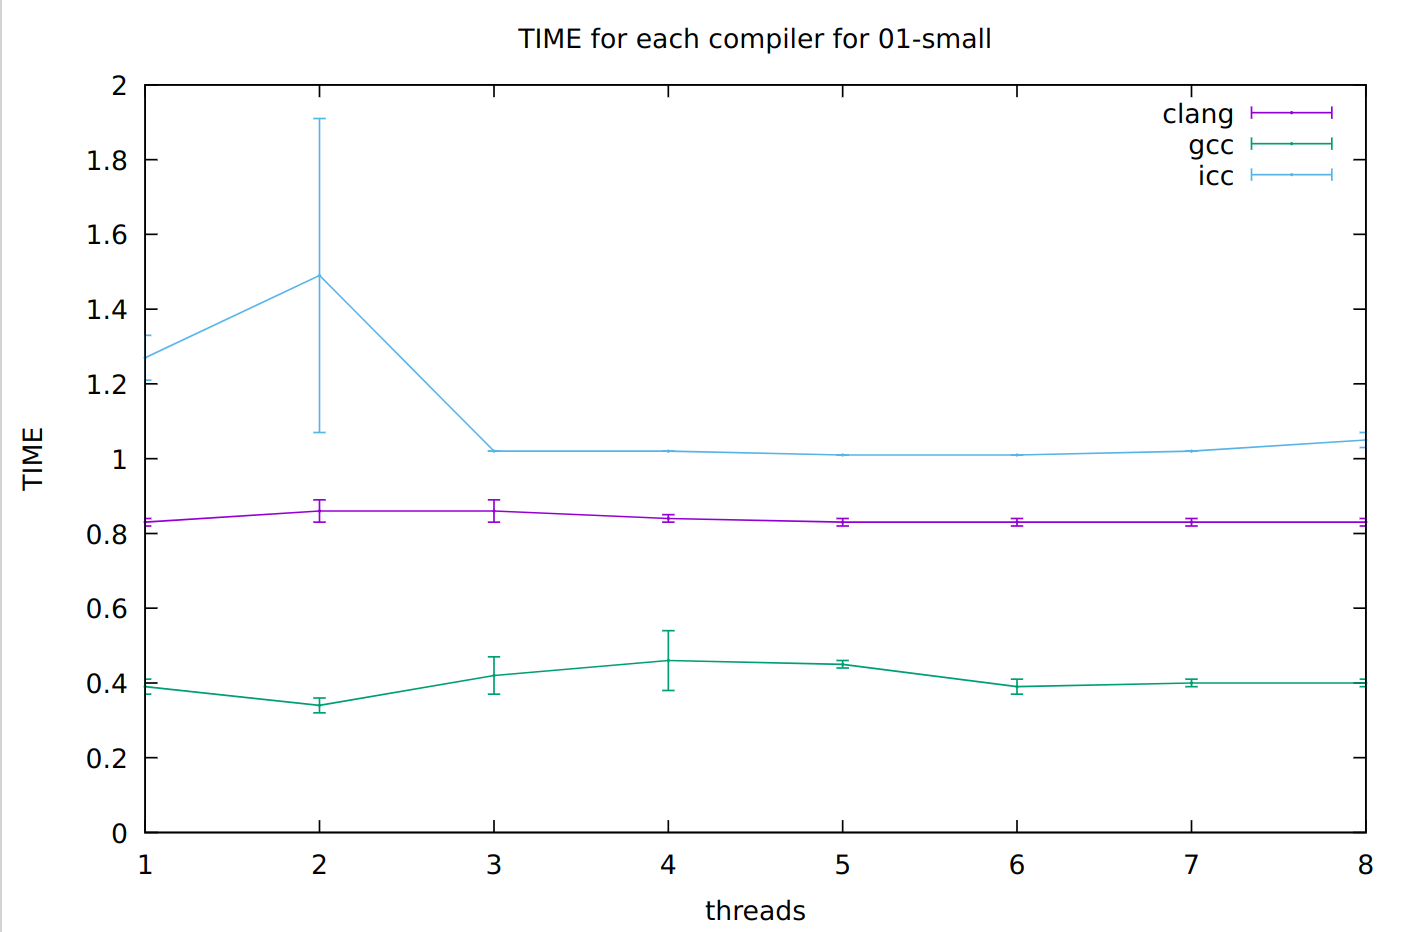
\includegraphics[width=\textwidth]{sin-cambios=01-small}
    \end{subfigure}
    \caption{\underline{Tamaño pequeño}: Tiempos de ejecución vs nº de hilos}
    \label{fig:sin-cambios=01-small}
\end{figure}

%%% TABLA DE TIEMPOS E IMÁGENES %%%
\begin{figure}[H]
    \centering
    \begin{subfigure}{0.4\textwidth}
        \begin{adjustbox}{width=\textwidth} 
        \begin{tabular}{|c|c|c|c|c|}
            \hline
            \rowcolor{azul} \multicolumn{2}{|c|}{}&\multicolumn{3}{c|}{\textbf{Compiler}} \\ \hline
            \rowcolor{azul} \multicolumn{2}{|c|}{}&\texttt{clang}&\texttt{gcc}&\texttt{icc}\\ \hline
            \rowcolor{azul} \textbf{Testing size} & \textbf{Threads}&\multicolumn{3}{c|}{\textbf{Average time (s)}} \\ \hline
            \multirow{8}{2.5cm}{\textbf{02-medium}} & 1 & \(2.38\pm{0.02}\) & \(1.15\pm{0.25}\) & \(2.91\pm{0.07}\) \\ \cline{2-5}
            & 2 & \(2.47\pm{0.10}\) & \(1.18\pm{0.24}\) & \(3.37\pm{0.39}\) \\ \cline{2-5}
            & 3 & \(2.38\pm{0.02}\) & \(1.33\pm{0.44}\) & \(2.93\pm{0.08}\) \\ \cline{2-5}
            & 4 & \(2.41\pm{0.05}\) & \(1.20\pm{0.31}\) & \(2.97\pm{0.12}\) \\ \cline{2-5}
            & 5 & \(2.42\pm{0.05}\) & \(1.20\pm{0.30}\) & \(2.96\pm{0.12}\) \\ \cline{2-5}
            & 6 & \(2.43\pm{0.06}\) & \(1.19\pm{0.29}\) & \(2.96\pm{0.12}\) \\ \cline{2-5}
            & 7 & \(2.38\pm{0.02}\) & \(1.87\pm{0.34}\) & \(2.93\pm{0.07}\) \\ \cline{2-5}
            & 8 & \(2.39\pm{0.03}\) & \(1.40\pm{0.25}\) & \(2.92\pm{0.07}\) \\ \hline
        \end{tabular}
        \end{adjustbox}
    \end{subfigure}
    \hfill
    \begin{subfigure}{0.5\textwidth}
        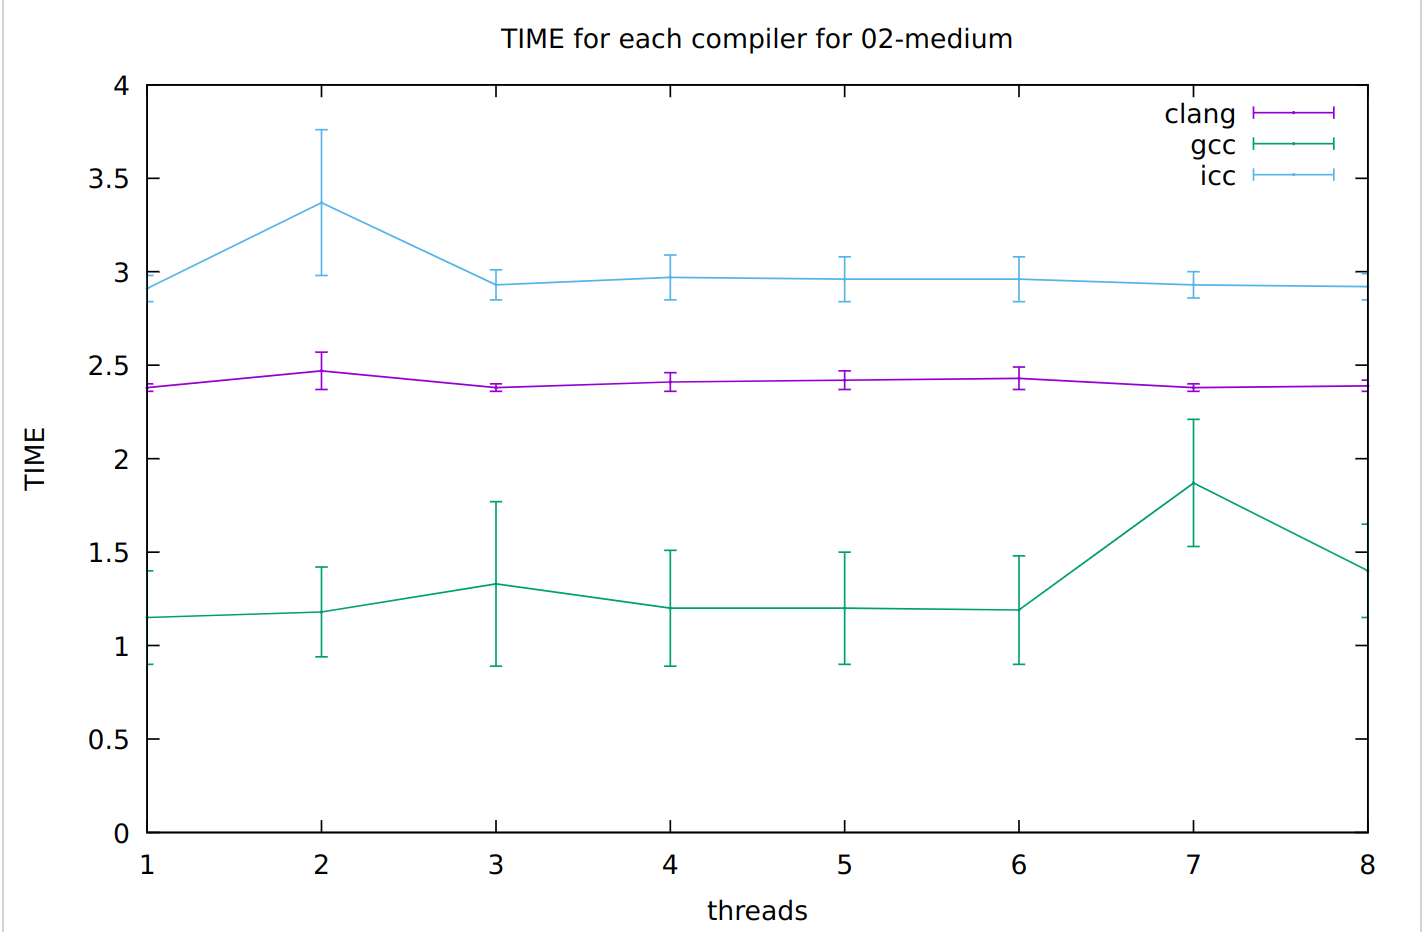
\includegraphics[width=\textwidth]{sin-cambios=02-medium}
    \end{subfigure}
    \caption{\underline{Tamaño mediano}: Tiempos de ejecución vs nº de hilos}
    \label{sin-cambios=02-medium}
\end{figure}

%%% TABLA DE TIEMPOS E IMÁGENES %%%
\begin{figure}[H]
    \centering
    \begin{subfigure}{0.4\textwidth}
        \begin{adjustbox}{width=\textwidth} 
        \begin{tabular}{|c|c|c|c|c|}
            \hline
            \rowcolor{azul} \multicolumn{2}{|c|}{}&\multicolumn{3}{c|}{\textbf{Compiler}} \\ \hline
            \rowcolor{azul} \multicolumn{2}{|c|}{}&\texttt{clang}&\texttt{gcc}&\texttt{icc}\\ \hline
            \rowcolor{azul} \textbf{Testing size} & \textbf{Threads}&\multicolumn{3}{c|}{\textbf{Average time (s)}} \\ \hline
            \multirow{8}{1cm}{\textbf{03-large}} & 1 & \(4.12\pm{0.08}\) & \(1.61\pm{0.12}\) & \(4.98\pm{0.15}\) \\ \cline{2-5}
            & 2 & \(4.10\pm{0.06}\) & \(1.61\pm{0.11}\) & \(4.94\pm{0.12}\) \\ \cline{2-5}
            & 3 & \(4.13\pm{0.09}\) & \(1.61\pm{0.12}\) & \(5.04\pm{0.20}\) \\ \cline{2-5}
            & 4 & \(4.10\pm{0.06}\) & \(1.60\pm{0.11}\) & \(4.95\pm{0.11}\) \\ \cline{2-5}
            & 5 & \(4.10\pm{0.06}\) & \(1.63\pm{0.12}\) & \(4.98\pm{0.15}\) \\ \cline{2-5}
            & 6 & \(4.16\pm{0.13}\) & \(1.60\pm{0.12}\) & \(4.94\pm{0.11}\) \\ \cline{2-5}
            & 7 & \(4.17\pm{0.11}\) & \(1.59\pm{0.12}\) & \(4.98\pm{0.15}\) \\ \cline{2-5}
            & 8 & \(4.15\pm{0.11}\) & \(1.60\pm{0.11}\) & \(4.95\pm{0.12}\) \\ \hline
        \end{tabular}
        \end{adjustbox}
    \end{subfigure}
    \hfill
    \begin{subfigure}{0.5\textwidth}
        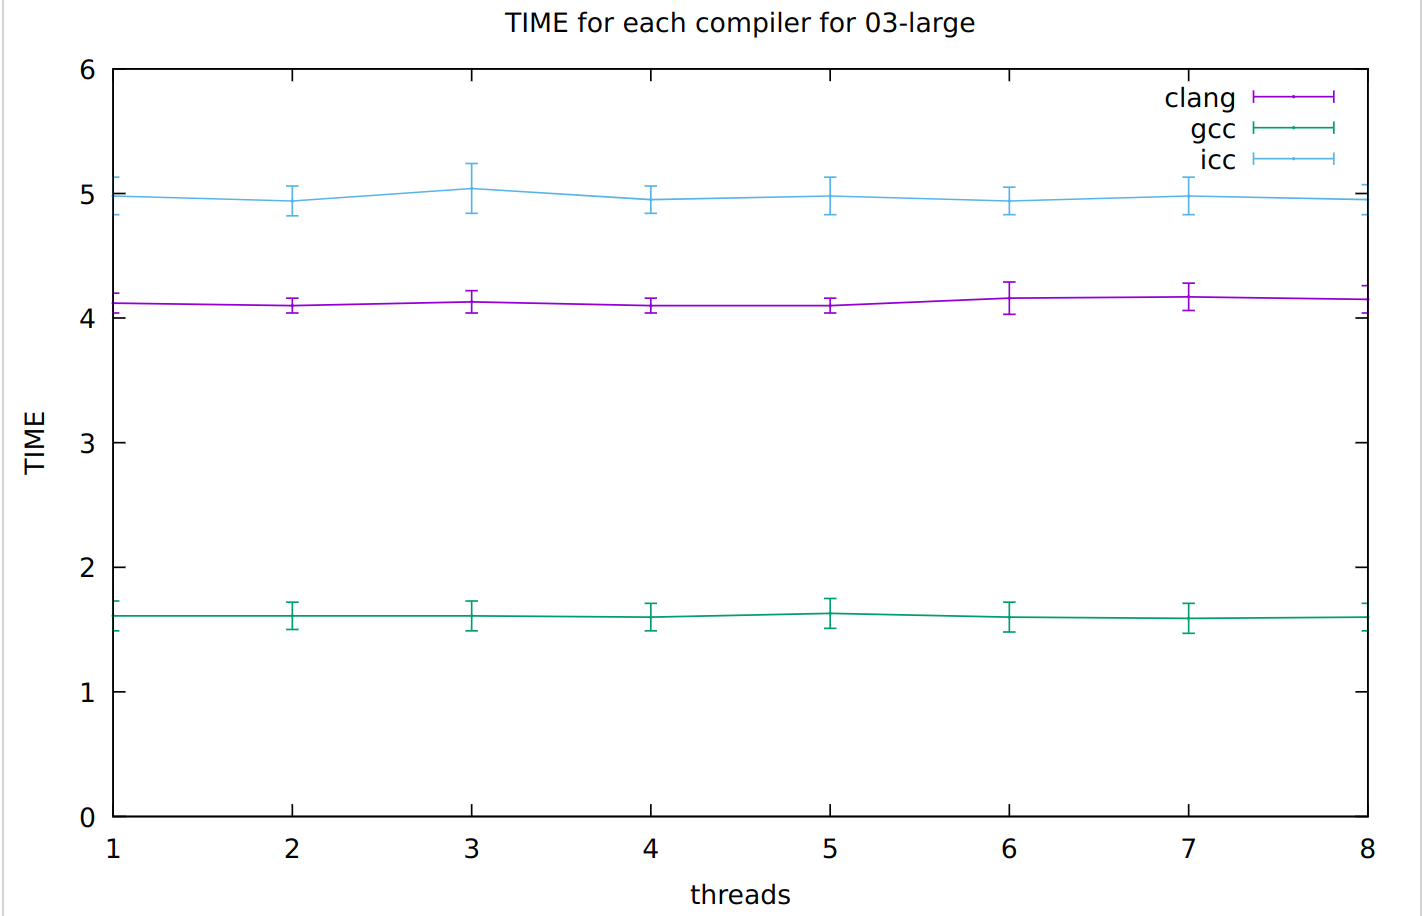
\includegraphics[width=\textwidth]{sin-cambios=03-large}
    \end{subfigure}
    \caption{\underline{Tamaño largo}: Tiempos de ejecución vs nº de hilos}
    \label{sin-cambios=03-large}
\end{figure}
